%%%%%%%%%%%%%%%%%%%%%%%%%%%%%%%%%%%%%%%%%
% University/School Laboratory Report
% LaTeX Template
% Version 3.1 (25/3/14)
%
% This template has been downloaded from:
% http://www.LaTeXTemplates.com
%
% Original author:
% Linux and Unix Users Group at Virginia Tech Wiki 
% (https://vtluug.org/wiki/Example_LaTeX_chem_lab_report)
%
% License:
% CC BY-NC-SA 3.0 (http://creativecommons.org/licenses/by-nc-sa/3.0/)
%
%%%%%%%%%%%%%%%%%%%%%%%%%%%%%%%%%%%%%%%%%

%----------------------------------------------------------------------------------------
%	PACKAGES AND DOCUMENT CONFIGURATIONS
%----------------------------------------------------------------------------------------

\documentclass[a4paper,12pt,notitlepage]{report}

\usepackage[version=3]{mhchem} % Package for chemical equation typesetting
\usepackage{siunitx} % Provides the \SI{}{} and \si{} command for typesetting SI units
\usepackage{graphicx} % Required for the inclusion of images
\usepackage{natbib} % Required to change bibliography style to APA
\usepackage{amsmath} % Required for some math elements 
\usepackage{listings}
\usepackage[utf8]{inputenc}
\usepackage[T1]{fontenc}
\usepackage{titlesec, blindtext, color}
\definecolor{gray75}{gray}{0.75}
\newcommand{\hsp}{\hspace{20pt}}
\titleformat{\chapter}[hang]{\Huge\bfseries}{\thechapter\hsp\textcolor{gray75}{|}\hsp}{0pt}{\Huge\bfseries}
[
\vspace{-2ex}
\textcolor{gray75}{\rule{\textwidth}{0.3pt}}
]

\titleformat{\section}[hang]{\Large\bfseries}{\thesection\hsp\textcolor{gray75}{|}\hsp}{0pt}{\Large\bfseries}

\setlength\parindent{0pt} % Removes all indentation from paragraphs

\renewcommand{\labelenumi}{\alph{enumi}.} % Make numbering in the enumerate environment by letter rather than number (e.g. section 6)

\newcommand{\HRule}{\rule{\linewidth}{0.5mm}}
%\usepackage{times} % Uncomment to use the Times New Roman font

\usepackage{xcolor}
\definecolor{dkgreen}{rgb}{0,0.6,0}
\definecolor{dred}{rgb}{0.545,0,0}
\definecolor{dblue}{rgb}{0,0,0.545}
\definecolor{lgrey}{rgb}{0.95,0.95,0.95}
\definecolor{gray}{rgb}{0.4,0.4,0.4}
\definecolor{darkblue}{rgb}{0.0,0.0,0.6}
\lstdefinelanguage{cpp}{
      backgroundcolor=\color{lgrey},  
      basicstyle=\footnotesize \ttfamily \color{black} \bfseries,   
      breakatwhitespace=false,       
      breaklines=true,               
      captionpos=b,                   
      commentstyle=\color{dkgreen},   
      deletekeywords={...},          
      escapeinside={\%*}{*)},                  
      frame=single,                  
      language=C++,                
      keywordstyle=\color{purple},  
      morekeywords={vec2,vec3,Vertex,string,mat4,Angel}, 
      identifierstyle=\color{darkblue},
      stringstyle=\color{orange},      
      numbers=left,                 
      numbersep=5pt,                  
      numberstyle=\tiny\color{blue}, 
      rulecolor=\color{orange},        
      showspaces=false,               
      showstringspaces=false,        
      showtabs=false,                
      stepnumber=1,                   
      tabsize=5,                     
      title=\lstname,                 
    }

%----------------------------------------------------------------------------------------
%	DOCUMENT INFORMATION
%----------------------------------------------------------------------------------------

\title{ \huge \bfseries Computer Graphics \\ \Large DTU 02561 (fall 2014) \\ REPORT } % Title
\author{Karol \textsc{Dzitkowski} s142246} % Author name
\date{\today} % Date for the report

\begin{document}

\maketitle % Insert the title, author and date
\HRule \\[1.5cm]
\begin{figure}[b]
	\begin{center}
		
\includegraphics{figures/DTU-logo}
	\end{center}
\end{figure}

\clearpage

\tableofcontents
\clearpage

% If you wish to include an abstract, uncomment the lines below
% \begin{abstract}
% Abstract text
% \end{abstract}

%----------------------------------------------------------------------------------------
%	CONTENT
%----------------------------------------------------------------------------------------

\chapter{Exercise 1}
The purpose of this exercise is to give a short introduction to
create, edit, link and run C/C++ programs that are based on the
graphics library OpenGL, and the utility libraries Angel and
GLUT.
\section{Part 1}
I drew another triangle by adding extra 3 vertices to the vertexData array:
\begin{figure}[ht!]
	\begin{center}
		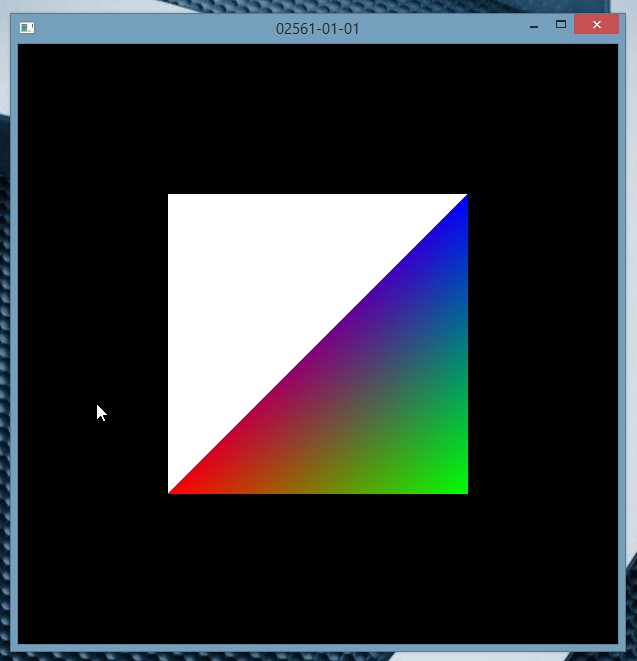
\includegraphics[width=0.5\textwidth]{figures/exercise_1_part_1}
	\end{center}
	\caption{Exercise 1 part 1 output}
\end{figure} \\
Below I described a meaning of each function used in a program:
\begin{description}
	\item[glGetAttribLocation] -- Returns the location of an attribute variable
	\item[glClearColor] -- specify clear values for the color buffers
	\item[glClear] -- clear buffers to preset values
	\item[glUseProgram] -- Installs a program object as part of current rendering state
	\item[glBindVertexArray] -- binds the vertex array object with name
	\item[glDrawArrays] -- render primitives from array data
	\item[glutSwapBuffers] -- swaps the buffers of the current window if double buffered
	\item[glViewport] -- sets the viewport
	\item[glGenVertexArrays] -- generate vertex array object names
	\item[glGenBuffers] -- generate buffer object names
	\item[glBindBuffer] -- bind a named buffer object
	\item[glBufferData] -- creates and initializes a buffer object's data store
	\item[glVertexAttribPointer] -- specify the location and data format of the array of generic vertex attributes at
	index index to use when rendering
	\item[Angel::InitShader] -- initializes shader programs stored in files passed as attributes
	\item[glutInit] -- initializes the GLUT library
	\item[glutInitContextVersion] -- sets openGL version we use
	\item[glutInitContextFlags] -- sets flags in GLUT library
	\item[glutInitContextProfile] -- sets profile of GLUT library
	\item[glutInitDisplayMode] -- sets the initial display mode
	\item[glutCreateWindow] -- creates a top-level window with a name passed as argument.
	\item[glutDisplayFunc] -- sets the display callback for the current window
	\item[glutReshapeFunc] -- sets the reshape callback for the current window
	\item[glutReshapeWindow] -- sets the window width and height
	\item[Angel::InitOpenGL] -- initializes OpenGL
	\item[glutMainLoop] -- enters the GLUT event processing loop
\end{description}


\section{Part 2}
I extended the program to include a triangle and rotated a rectangle using code below:
\begin{lstlisting}[language=cpp, caption={Exercise 1 part 1 code changes}]
void loadGeometry(){
// add a triangle
Vertex triangleData[triangleSize] = {
	{ vec2(2,2), vec3(1.0, 0.0, 0.0) },
	{ vec2(5,2), vec3(0.0, 1.0, 0.0) },
	{ vec2(3.5,5), vec3(0.0, 0.0, 1.0) }};
triangleVertexArrayBuffer = loadBufferData(triangleData, triangleSize);}

void display(){
// to rotate rectangle
mat4 modelView2 = Angel::RotateZ(45);
glUniformMatrix4fv(modelViewUniform, 1, GL_TRUE, modelView2);
// transform and render the triangle
mat4 modelView;
modelView[0][3]=6;
modelView[1][3]=7;
modelView[2][3]=0;
glUniformMatrix4fv(modelViewUniform, 1, GL_TRUE, modelView);
glBindVertexArray(triangleVertexArrayBuffer);
glDrawArrays(GL_TRIANGLE_FAN, 0, triangleSize);}
\end{lstlisting}
After applying these changes I got an output: \\
\begin{figure}[ht!]
	\begin{center}
		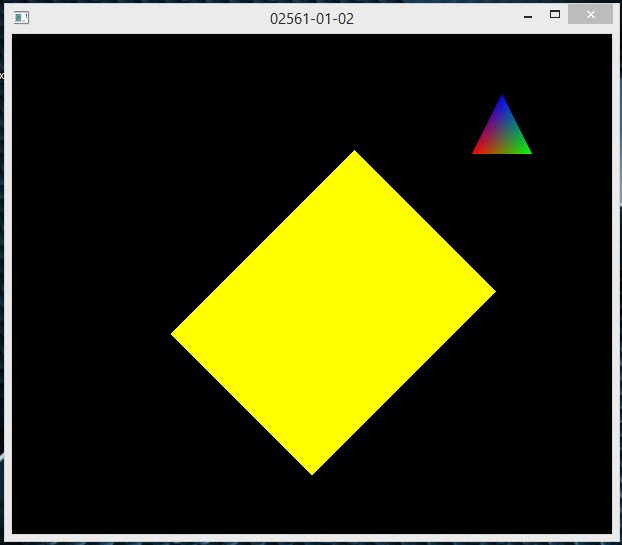
\includegraphics[width=0.45\textwidth]{figures/exercise_1_part_2}
	\end{center}
	\caption{Exercise 1 part 2 output}
\end{figure}


\section{Part 3}
\subsection{glDrawArrays vs glDrawElements}
The nvidia docs say that glDrawElements is faster because of potential vertex sharing.
Function glDrawArrays submits the vertices in linear order, as they are stored in the vertex arrays.
With glDrawElements one has to supply an index buffer. Indices allow to submit the vertices in any 
order, and to reuse vertices that are shared between triangles.
\subsection{Triangle rendering types}
\begin{description}
	\item[GL\_TRIANGLES] - A triangle is composed from every three vertices. First is composed 
	from vertives $(0,1,2)$ second from $(3,4,5)$ and so on. 
	\item[GL\_TRIANGLE\_STRIP] - Draws a series of triangles using vertices $(0,1,2)$ then $(2,1,3)$ then
	$(2,3,4)$ and so on. The ordering is to ensure that the triangles are all drawn with the same
	orientation so that the strip can correctly form part of a surface.
	\item[GL\_TRIANGLE\_FAN] - The first vertex is always held fixed. From there on, every group of
	2 adjacent vertices form a triangle with the first.
\end{description}
\subsection{Extended program}
Below I present an output of the extended program:
\begin{figure}[ht!]
	\begin{center}
		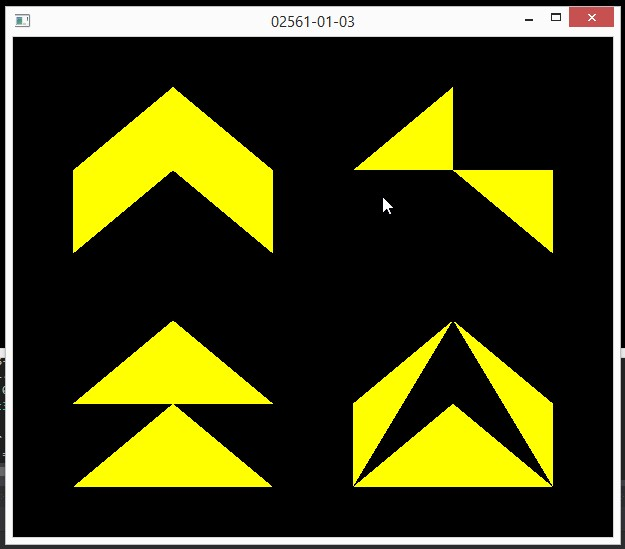
\includegraphics[width=0.45\textwidth]{figures/exercise_1_part_3}
	\end{center}
	\caption{Exercise 1 part 3 output}
\end{figure} 
\clearpage


\section{Part 4}
The resulting screenshot of program extension can be seen in Figure \ref{fig:exercise_1_part_4} \\
\begin{figure}[ht!]
	\begin{center}
		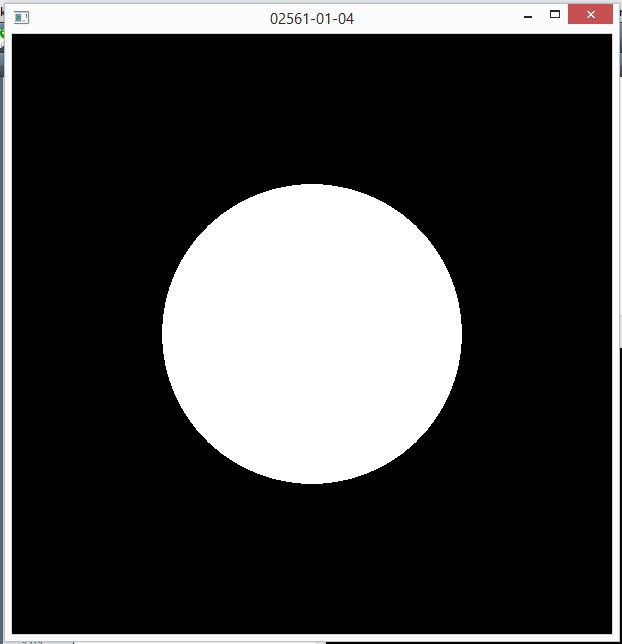
\includegraphics[width=0.5\textwidth]{figures/exercise_1_part_4}
	\end{center}
	\caption{Exercise 1 part 4 output}
	\label{fig:exercise_1_part_4} 
\end{figure} \\
I did it using GL\_TRIANGLE\_FAN option in glDrawArrays and created vertices in vertexData using code:
\begin{lstlisting}[language=cpp, caption={Exercise 1 part 4 creating circle vertices}]
void loadBufferData() {
	for (int i=1; i < NUMBER_OF_VERTICES; i++)
	{
		float const t = 2*M_PI*(float)i/(float)(NUMBER_OF_VERTICES - 2);
		vertexData[i].x = origin.x + cos(t)*CIRCLE_RADIUS;
		vertexData[i].y = origin.y + sin(t)*CIRCLE_RADIUS; 
	}
	//...
}
\end{lstlisting}
\clearpage
\section{Part 5}
I succeeded to draw the figure by using scaling, rotation and transforming from Angel library and
glDrawArrays function with GL\_TRIANGLES option.
For example printing inside triangles is done using code:
\begin{lstlisting}[language=cpp, caption={Exercise 1 part 5 inside triangles}]
mat4 innerTriangleModelView = Angel::Scale(10,10,10);
innerTriangleModelView *= Angel::RotateX(180);

for(int i=0; i<4; i++)
{
	glUniformMatrix4fv(modelViewUniform, 1, GL_TRUE, innerTriangleModelView);
	glDrawArrays(GL_TRIANGLES, 0, NUMBER_OF_VERTICES);
	innerTriangleModelView *= Angel::RotateZ(90);
}
\end{lstlisting}
\begin{figure}[ht!]
	\begin{center}
		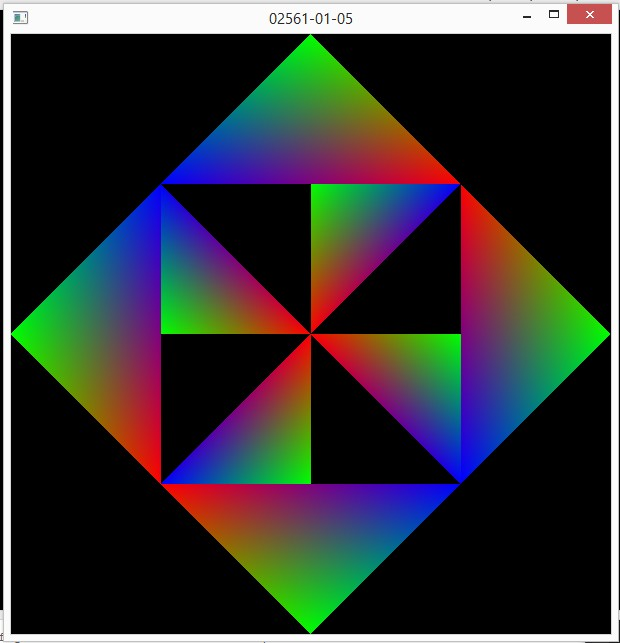
\includegraphics[width=0.5\textwidth]{figures/exercise_1_part_5}
	\end{center}
	\caption{Exercise 1 part 5 output}
	\label{fig:exercise_1_part_5} 
\end{figure}
\clearpage

\section{Part 6}
Transformation matrix which maps a point $(xw,yw)$ to the point $(xv,yv)$ considering a
window - viewport pair as 
$$
w = [w_{x_{min}},w_{x_{max}},w_{y_{min}},w_{y_{max}}],
v = [v_{x_{min}},v_{x_{max}},v_{y_{min}},v_{y_{max}}]
$$
looks like that:
\begin{align*}
M_{wv} =
  \begin{bmatrix}
    \dfrac{v_{x_{max}} - v_{x_{min}}}{w_{x_{max}} - w_{x_{min}}} & 0 & v_{x_{min}}
    - w_{x_{min}} \cdot \dfrac{v_{x_{max}} - v_{x_{min}}}{w_{x_{max}} - w_{x_{min}}} \\
    0 & \dfrac{v_{y_{max}} - v_{y_{min}}}{w_{y_{max}} - w_{y_{min}}} & v_{y_{min}}
    - w_{y_{min}} \cdot \dfrac{v_{y_{max}} - v_{y_{min}}}{w_{y_{max}} - w_{y_{min}}} \\
    0 & 0 & 1
  \end{bmatrix}
\end{align*}

And is a concatenation of three transformations:
$$
M_{wv} = T_{1}(v_{x_{min}},v_{y_{min}}) \cdot S(s_x, s_y) \cdot T_{2}(w_{x_{min}}, w_{y_{min}})
$$
\begin{itemize}
	\item Translation
		\begin{align*}
		T_{1} =
      \begin{bmatrix}
          1 & 0 & v_{x_{min}} \\
          0 & 1 & v_{y_{min}} \\
          0 & 0 & 1
      \end{bmatrix} 
		\end{align*}
	\item Scaling
		\begin{align*}
    	S =
      \begin{bmatrix}
          \dfrac{v_{x_{max}} - v_{x_{min}}}{w_{x_{max}} - w_{x_{min}}} & 0 & 0 \\
          0 & \dfrac{v_{y_{max}} - v_{y_{min}}}{w_{y_{max}} - w_{y_{min}}} &  0 \\
          0 & 0 & 1
      \end{bmatrix} 
		\end{align*}
	\item Translation
		\begin{align*}
    	T_{2} =
      \begin{bmatrix}
          1 & 0 & -w_{x_{min}} \\
          0 & 1 & -w_{y_{min}} \\
          0 & 0 & 1
        \end{bmatrix} 
		\end{align*}
\end{itemize}
Multiplication of these 3 transformation matrices gives the window-viewport transformation matrix.
In OpenGL glViewport() command is used to define the rectangle of the rendering area where the
final image is mapped.
\clearpage

\section{Part 7}
I rendered a Sierpinski carpet using a recursive function I wrote, below is an output for 6 iterations:
\begin{figure}[ht!]
	\begin{center}
		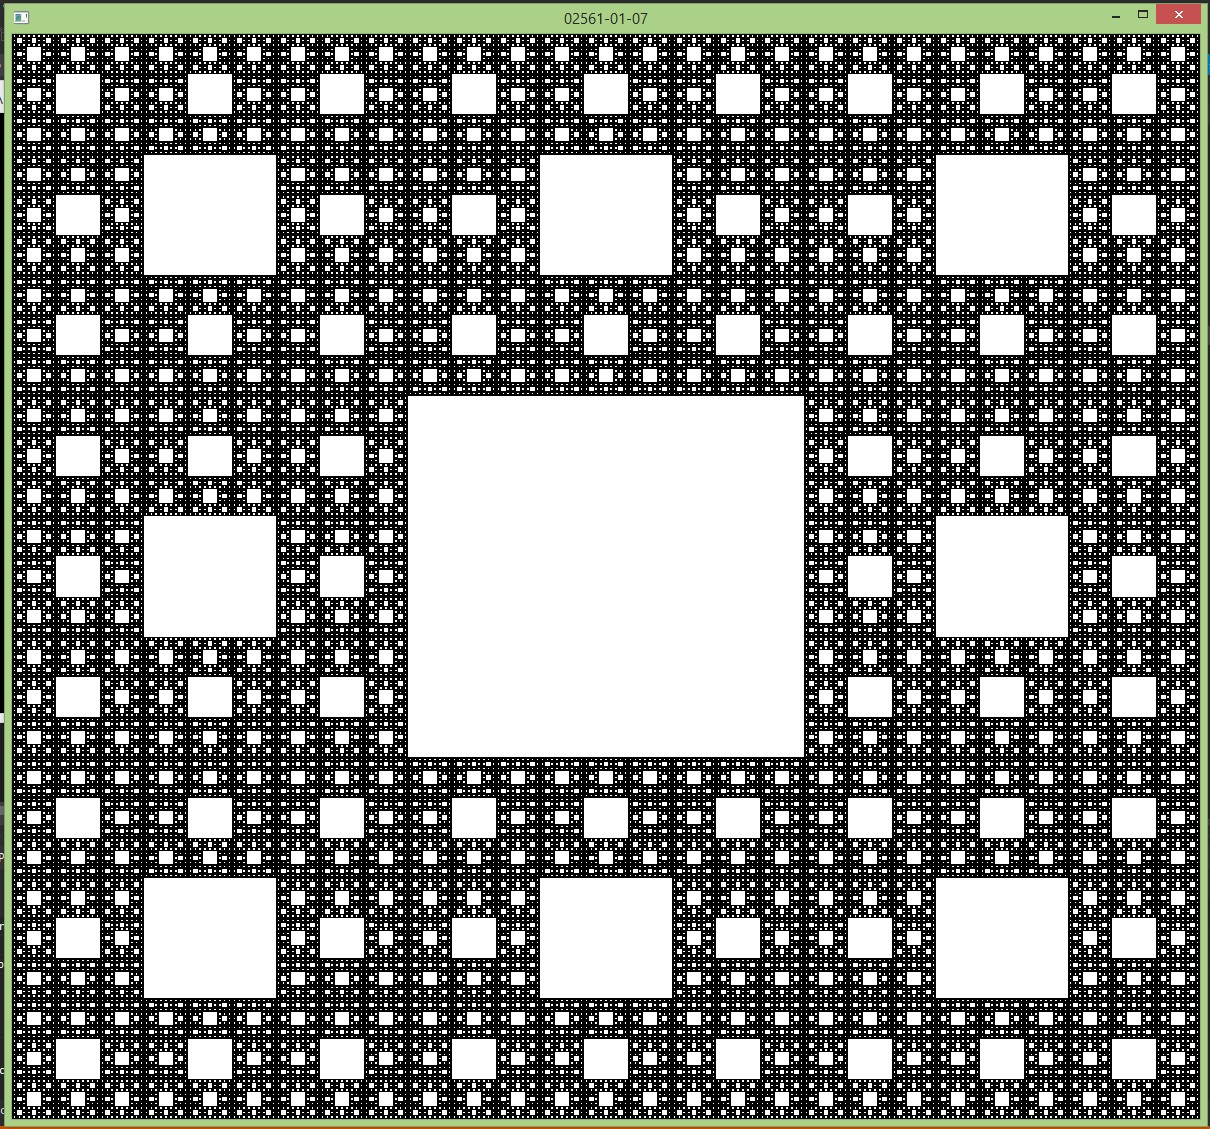
\includegraphics[width=0.5\textwidth]{figures/exercise_1_part_7}
	\end{center}
	\vspace{-4.5ex}\caption{Exercise 1 part 7 output}
	\label{fig:exercise_1_part_7} 
\end{figure} \\
As an input the function which generates points takes vertives of the biggest square. We will also get
an interesting fractal when we switch the order of the vertices (Figure \ref{fig:exercise_1_part_7_extra}).
\begin{lstlisting}[language=cpp, caption={Exercise 1 part 7 point gen.}]
vec2 vertices[4] = {vec2(-1.0, -1.0), vec2(-1.0, 1.0), vec2(1.0, -1.0), vec2(1.0, 1.0)};
divide_square(vertices[0], vertices[1], vertices[2], vertices[3], NumTimesToSubdivide);
\end{lstlisting}
\begin{figure}[ht!]
	\begin{center}
		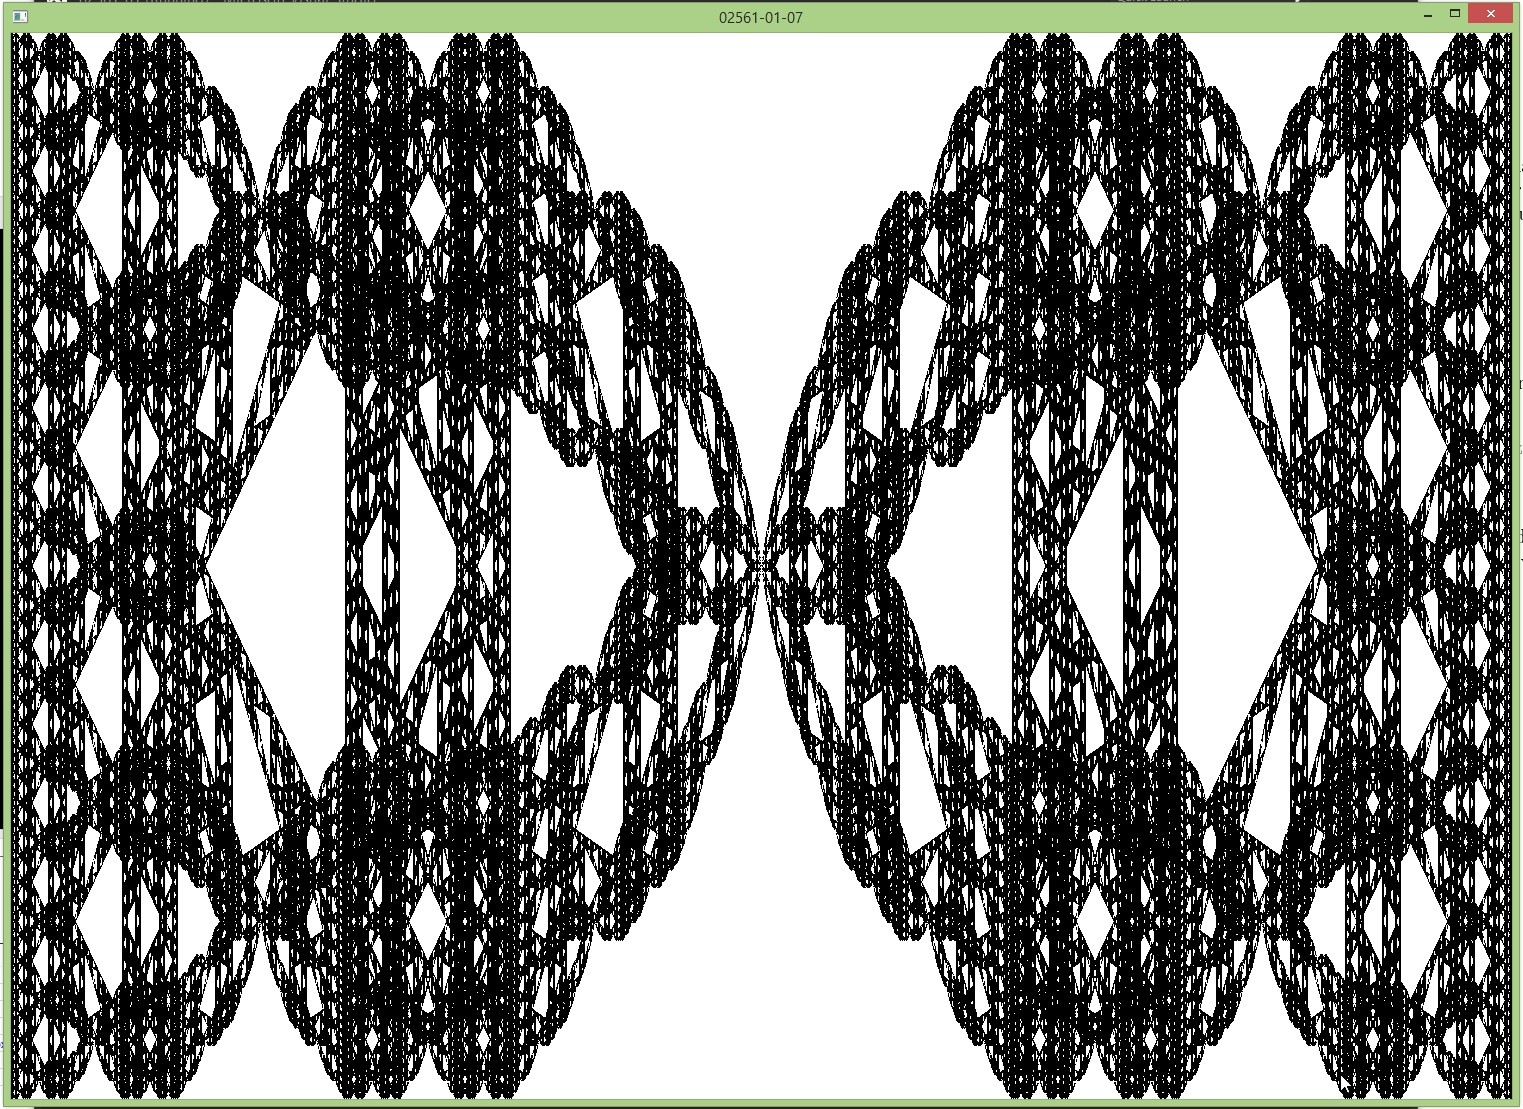
\includegraphics[width=0.5\textwidth]{figures/exercise_1_part_7_extra}
	\end{center}
	\vspace{-4.5ex}\caption{Exercise 1 part 7 output (vertices order changed)}
	\label{fig:exercise_1_part_7_extra} 
\end{figure}
\chapter{Exercise 2}
The purpose of this exercise is to understand the various method of setting up
the virtual camera and to be able to adjust the parameters of the camera. We will
get more acquainted with defining the matrices in the viewing pipeline and to
concatenate them into the viewing matrix. Secondly, we will make different
pictures of the scene using various projection method based on central projection
(Front, X and 3-point perspective) and Orthographic parallel projection
(Isometric, Dimetric, and Trimetric axonometric).


\section{Part 1}
\begin{itemize}
\item Vertex structure in Exercise 1 was represented by a pair of 2D cartesian coordinates
as vec2 and a color as vec3. On the other hand in Exercise 2 vertices are points in
3D space so they are represented in homogenous coordinates as vec4.
\item In Exercise 1 in display function we defined an Ortho2D projection and we were describing
model-view properties of our vision. In this exercise we use Ortho (3D) projection and we use
a LookAt function which takes an eye position, an up vector, and look at positon, which does
a camera inverse transformation (creates a modelView matrix).
\end{itemize}
\clearpage

\section{Part 2}
To produce a required output I used 3 transformations in an order:
\begin{enumerate}
\item Translation
\item Scaling
\item Rotation around Y axis
\end{enumerate}
\begin{lstlisting}[language=cpp, caption={Transformations}]
modelView *= Angel::Translate(0,3,0);
modelView *= Angel::Scale(2,2,2);
modelView *= Angel::RotateY(30);
\end{lstlisting}
An output for this order of transformation can be seen in Figure \ref{fig:exercise_2_part_2},
however if we change the order of transformations for example make Translate the last operation,
we can get different output, because matrix multiplication isn't a commutative operation.
\begin{figure}[ht!]
	\begin{center}
		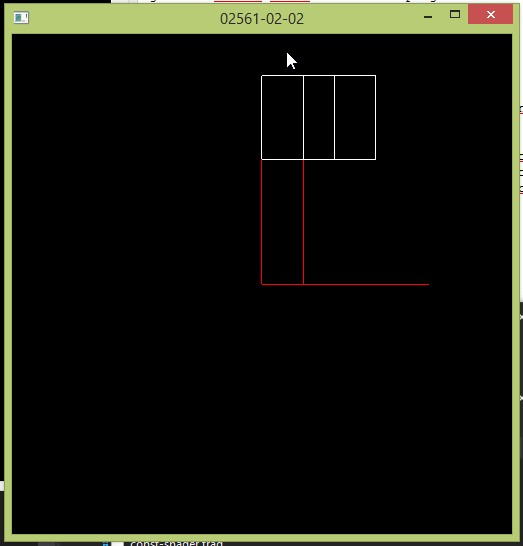
\includegraphics[width=0.5\textwidth]{figures/exercise_2_part_2}
	\end{center}
	\caption{Exercise 2 part 2 output}
	\label{fig:exercise_2_part_2} 
\end{figure}
\clearpage


\section{Part 3}
Following the instructions in the exercise part 2 gave me an expected result which can be seen below:
\begin{figure}[ht!]
	\begin{center}
		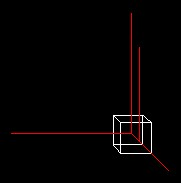
\includegraphics[width=0.5\textwidth]{figures/exercise_2_part_3}
	\end{center}
	\caption{Exercise 2 part 3 output}
	\label{fig:exercise_2_part_3} 
\end{figure} \\
To aquire this I used the following code:
\begin{lstlisting}[language=cpp, caption={Front perspective projection}]
mat4 projection = Angel::Perspective(45, 1, 1, 100);
glUniformMatrix4fv(projectionUniform, 1, GL_TRUE, projection);
vec3 eye(20, 5, 5);
vec3 up(0, 1, 0);
vec3 at(0, 5, 5);
mat4 modelView = Angel::LookAt(eye, at, up);//*Angel::Scale(3,3,3);
\end{lstlisting}
\clearpage


\section{Part 4}
I succeeded in creating an isometric view using code below, the results are shown in Figure \ref{fig:exercise_2_part_4}
\begin{lstlisting}[language=cpp, caption={Front perspective projection}]
mat4 projection = Ortho(-6., 6., -6., 6., -6., 10.);
glUniformMatrix4fv(projectionUniform, 1, GL_TRUE, projection);
vec3 eye(5,5,5);
vec3 at(0,0,0);
vec3 up(0,0,1);
mat4 modelView = Angel::LookAt(eye, at, up);
\end{lstlisting}
\begin{figure}[ht!]
	\begin{center}
		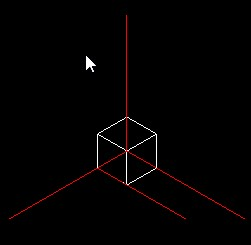
\includegraphics[width=0.5\textwidth]{figures/exercise_2_part_4}
	\end{center}
	\caption{Exercise 2 part 4 output}
	\label{fig:exercise_2_part_4} 
\end{figure}



\section{Part 5}
I managed to get the same results using corresponding code parts:
\begin{lstlisting}[language=cpp, caption={Rotation and translation 1}]
// view = LookAt(vec4(-.5, 1, 6,1), vec4(-2,1,0,1), vec4(0,1,0,0));
view = RotateY(-atan(1.5/6.0)/DegreesToRadians) * Translate(.5, -1, -6);
\end{lstlisting}
\begin{lstlisting}[language=cpp, caption={Rotation and translation 2}]
// view = RotateY(-120) * Translate(-4, -1, -1);
vec3 eye(4, 1, 1);
vec3 at(4-sqrt(3), 1, 2);
vec3 up(0,1,0);
view = LookAt(eye, at, up);
\end{lstlisting}
\begin{lstlisting}[language=cpp, caption={Rotation and translation 3}]
// view = LookAt(vec4(-1, 1, 9,1), vec4(-1,1,0,1), vec4(0,1,0,0));
view = mat4(
	1,0,0,0,
	0,1,0,0,
	0,0,1,0,
	1,-1,-9,1
	);
\end{lstlisting}


\section{Part 6}
\begin{description}
  \item[Part 1 transformation]
  	$$\emph{Angel::RotateX(atan(3/6)/DegreesToRadians)*Angel::Translate(0,-3,-6);}$$
  \item[Part 2 transformation]
  	$$\emph{Angel::Translate(0,3,0)*Angel::RotateY(30)*Angel::Scale(2,2,2);}$$
\end{description}

\chapter{Exercise 3}
In this part we setup both shader uniformas and vertex attributes in both shader code and C++ code.
This is also an introduction to a very simple type of animation called vertex blending performed in
the vertex shader using GLSL.

\section{Part 1 and 2}
In the figure \ref{fig:exercise_3_part_1} we can see how vertex blending works in the program.

\begin{figure}[ht!]
	\begin{center}
		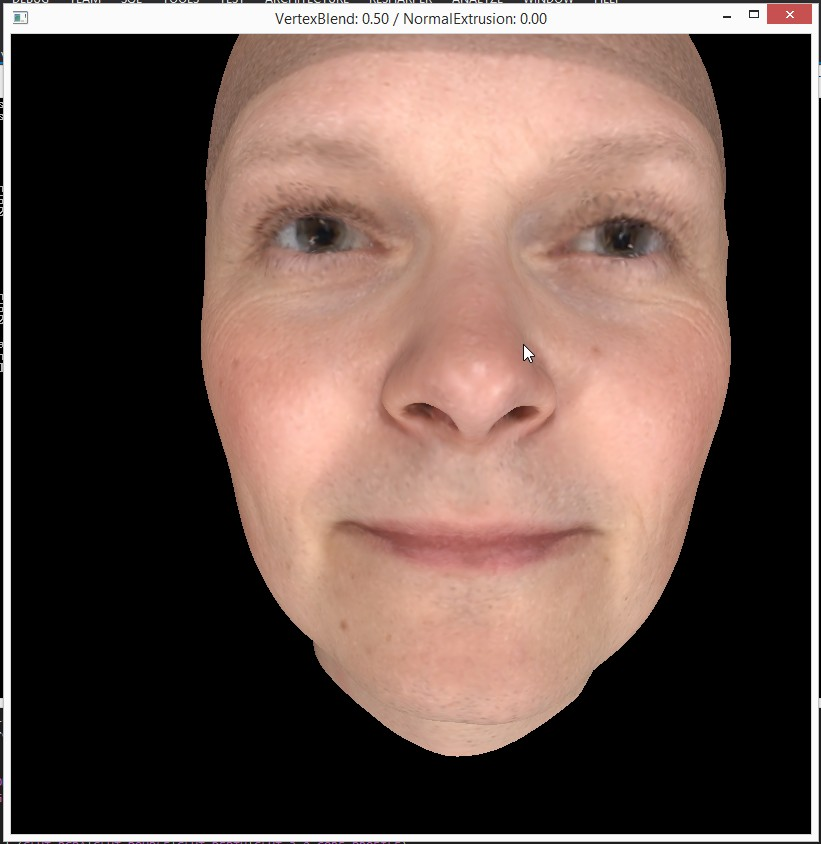
\includegraphics[width=0.5\textwidth]{figures/exercise_3_part_1}
	\end{center}
	\vspace{-4.5ex}\caption{Exercise 3 part 1 output}
	\label{fig:exercise_3_part_1} 
\end{figure}
I also modified the vertex shader to move the vertex along the normal direction by the amount specified
by normalExtrusion. This can be seen in the figure \ref{fig:exercise_3_part_2}.
\clearpage
\begin{figure}[ht!]
	\begin{center}
		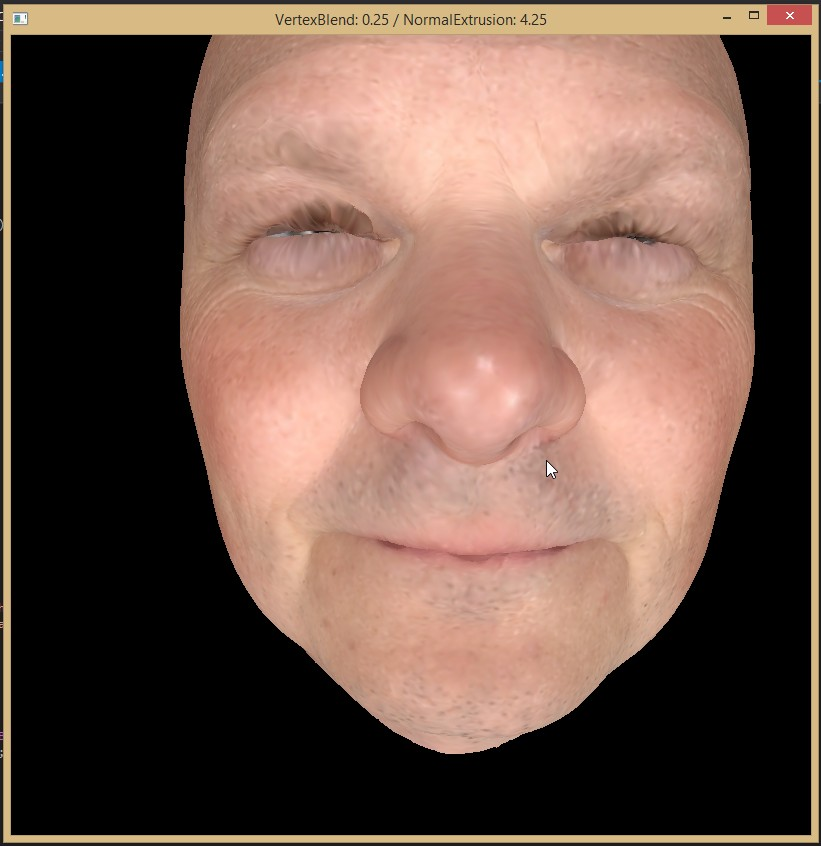
\includegraphics[width=0.5\textwidth]{figures/exercise_3_part_2}
	\end{center}
	\vspace{-4.5ex}\caption{Exercise 3 part 2 output}
	\label{fig:exercise_3_part_2} 
\end{figure}

All this transformations are done by the code in vertex shader:

\begin{lstlisting}[language=cpp, caption={Vertex blending}]
uniform mat4 projection;
uniform mat4 modelView;
uniform float blendValue;
uniform float normalExtrusion;

in vec3 position1;
in vec3 color1;
in vec3 position2;
in vec3 color2;
in vec3 normal1;
in vec3 normal2;

out vec3 colorV;
out vec3 position;

void main (void) {
	vec3 blendVector = vec3(blendValue);
    colorV = (1 - blendVector) * color1 + (blendVector * color2);
	vec3 normal = (1 - blendVector) * normal1 + (blendVector * normal2);
	position = (1 - blendVector) * position1 + (blendVector * position2) + (normal * normalExtrusion);
	gl_Position = projection * modelView * vec4(position, 1.0);
}
\end{lstlisting}
\clearpage

\section{Part 3}
\begin{description}
\item[Difference between a vertex attribute and a vertex uniform]
	Vertex attribute is a ,,vector'' of values, specified for each vertex, 
	while uniforms are sort of ,,constant'' values - the same value for all the vertices. 
	Both can be changed between the callbacks of a drawing function. 
\item[Vertex shader]
	The vertex shader manipulates the attributes of vertices, which are the corner points of displayed objects.
	It is a part of the early steps in the pipline where transforming of vertex location from one coordinate
	system to another is done. It computes the representation of a vertex in clip coordinates for the rasterizer.
\item[Fragment shader]
	The fragment shader takes care of how the pixels between the vertices look like (their color).
	Is is a part of rasterization step, where pixels between the vertices are coloured. 
\item[Between vertex shader and the fragment shader]
	Pixels are usually interpolated between the defined vertices in vertex shader following specific rules
	and passed through to the fragment shader.
\item[Blending the color in the fragment shader]
	It is possible and it is usually done there to obtain better quality. There is a special function for blending
	called mix, and it will be done per pixel not per vertex. However doing it in fragment shader can result in 
	lower performance.
\end{description}
\clearpage

\section{Part 3}
As it can be seen in the figure \ref{fig:exercise_3_part_3} I successfully obtained working 
discarding all pixels with even y coordinate using the code below.

\begin{lstlisting}[language=cpp, caption={Discarding pixels}]
in vec3 colorV;
in vec3 position;
out vec4 fragColor;

void main(void)
{
	if (mod(round(position.y),2) == 0) discard;
    fragColor = vec4(colorV, 1.0);
}
\end{lstlisting}

\begin{figure}[ht!]
	\begin{center}
		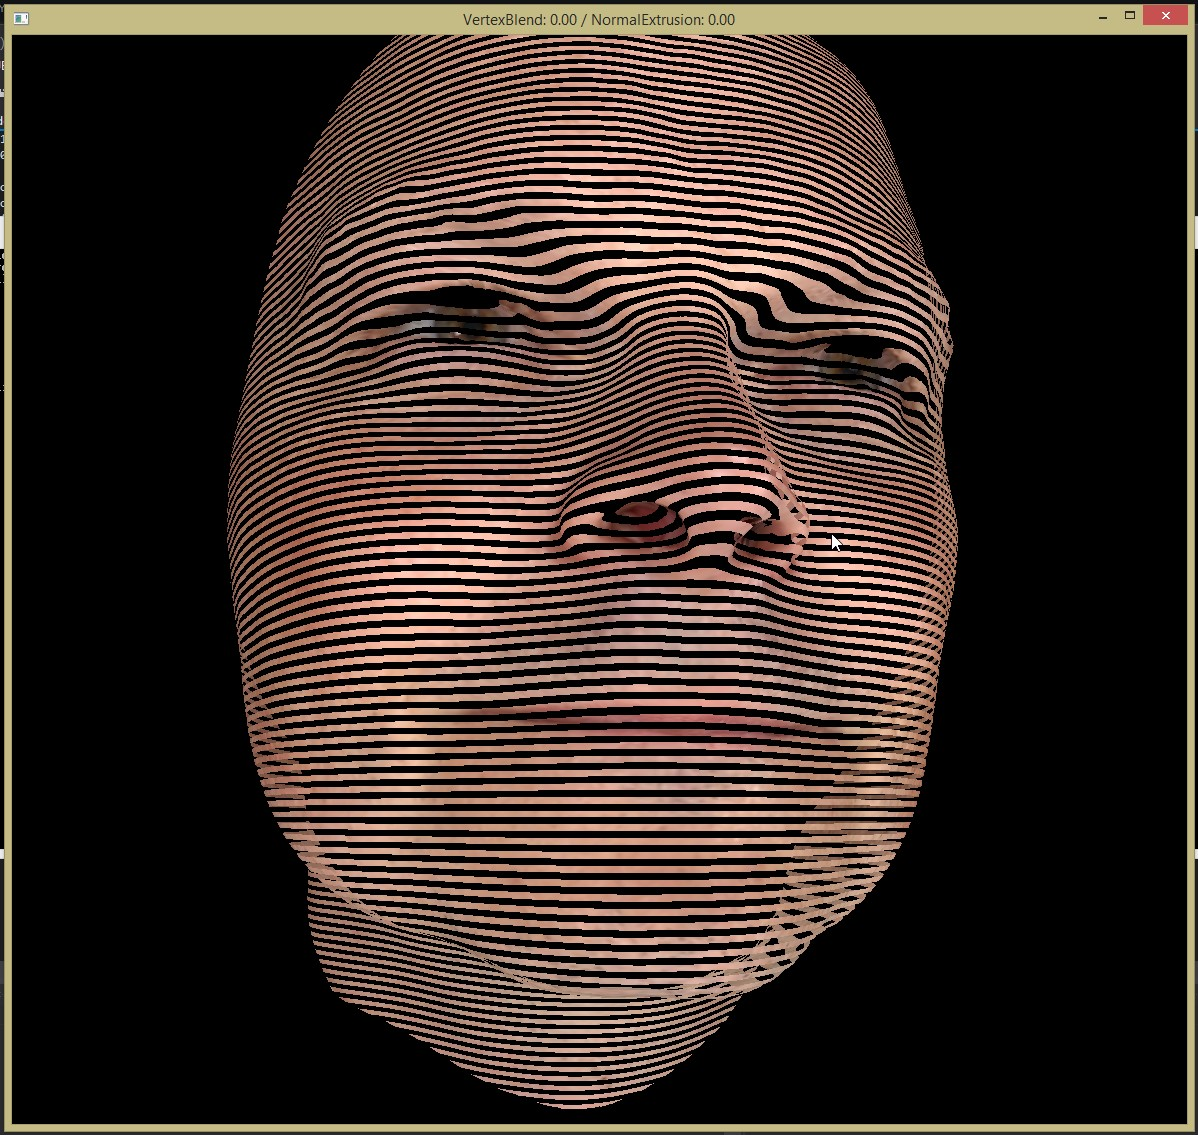
\includegraphics[width=0.9\textwidth]{figures/exercise_3_part_3}
	\end{center}
	\vspace{-4.5ex}\caption{Exercise 3 part 3 output}
	\label{fig:exercise_3_part_3} 
\end{figure}


\chapter{Exercise 4}
The purpose of this exercise is to get acquainted with lighting and
shading in OpenGL and GLSL.
You will calculate the shading of an object based on the ambient,
diffuse and specular properties of the material and the light source.

\section{Part 1}
I successfully modified the vertex shader to implement Phong ligthing using Gouraud
which can be seen in figure \ref{fig:exercise_4_part_1}
\begin{figure}[ht!]
	\begin{center}
		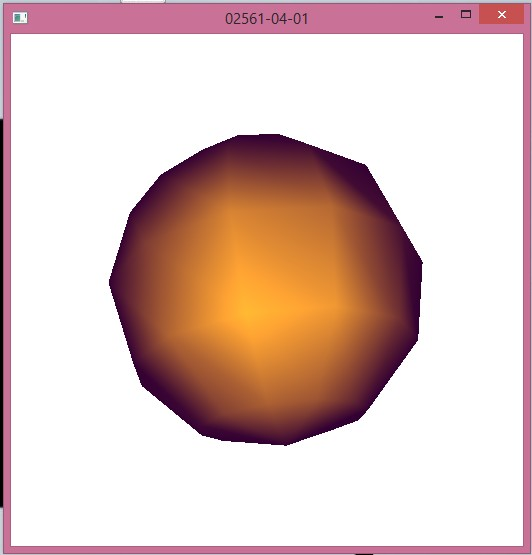
\includegraphics[width=0.5\textwidth]{figures/exercise_4_part_1}
	\end{center}
	\vspace{-4.5ex}\caption{Exercise 4 part 1 output}
	\label{fig:exercise_4_part_1} 
\end{figure}

\section{Part 2}
In the pictures below 
(figures \ref{exercise_4_part_2-1} and \ref{exercise_4_part_2-2}) 
you can see implemented
Phong shading using fragment shader also with specular contribution.
\begin{figure}[ht!]
	\begin{center}
		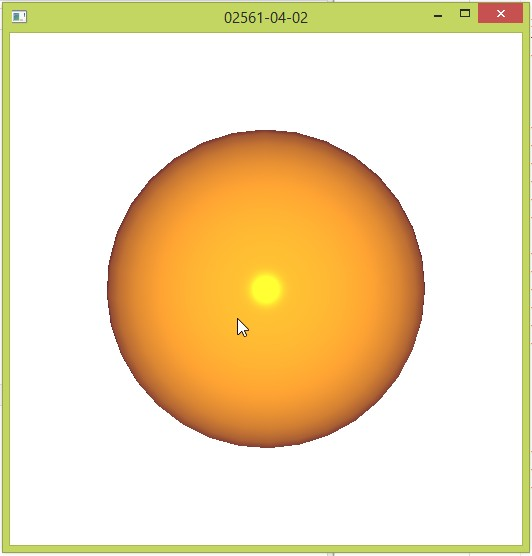
\includegraphics[width=0.6\textwidth]{figures/exercise_4_part_2-1}
	\end{center}
	\vspace{-4.5ex}\caption{Exercise 3 part 2 output (directional)}
	\label{fig:exercise_4_part_2-1} 
\end{figure}
\begin{figure}[ht!]
	\begin{center}
		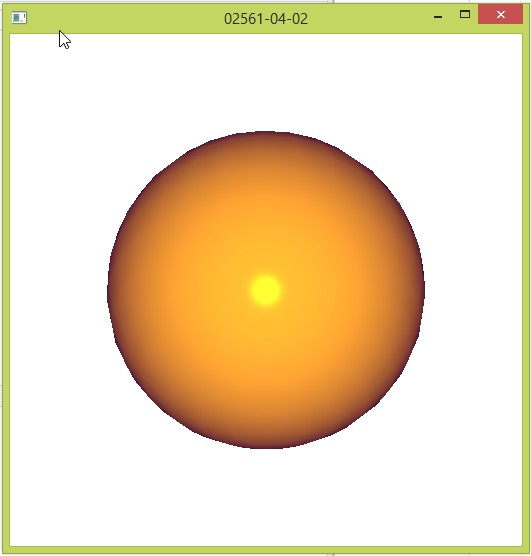
\includegraphics[width=0.6\textwidth]{figures/exercise_4_part_2-2}
	\end{center}
	\vspace{-4.5ex}\caption{Exercise 4 part 2 output (point)}
	\label{fig:exercise_4_part_2-2} 
\end{figure}
\clearpage

\section{Part 3}
\begin{description}
\item[Phong shading and Phong lighting]
	Phong lightning is a model of lightning where object surface is covered by thin transparent layer,
	where specular reflection takes place. While Phong shading is a technique of shading the polygons,
	where a normal vector is interpolated between vertices and then any lightning model is used for 
	interpolated pixels. 
\item[Gouraud shading and Phong shading]
	This two shading methods differs how a normal vector is assigned to pixels when calculating a color.
	In Goroaud shading color is calculated for every vertex using its normal vector, and then color is
	interpolated, while in Phong shading normal vector is interpolated and color is calculated for each pixel.
	Goraud shading is faster but less accurate than Phong shading.
\item[Point light and directional light]
	In directional light, rays are parallel to each other.
\item[Eye position any influence]
	Eye position is substantial in rendering reflections of the light from shiny objects.
\item[Specular term equal to $(0,0,0)$]
	The reflection disappeares.
\item[Increasing shininess exponent]
	When shininess exponent is inceased the reflection is getting smaller and it is more simillar to a perfect mirror.
\item[Simplifications] No simplifications were used.
	
\item[Normal matrix]
	Normal matrix is used to transform the normal into eye space. We only want to transform its orientation. 
	The region of the modelview matrix that contains the orientation is the top left $3*3$ submatrix. The reason
	of using normalized matrix is that a modelview matrix can contain a non-uniform scale. Because of that we
	compute this matrix as:
	\begin{lstlisting}[language=cpp, caption={Normal matrix}]
	normalize(transpose(inverse(mat3(ModelView))) * fragNormal);
	\end{lstlisting}
\item[Light coordinate space]
	I use eye space coordinate system because it is easier to calculate specular light effect.
\end{description}
\clearpage

\section{Part 4}
I implemented Phong shading for multiple light sources with different colors and attributes.
It is done using code below in the fragment shader and the results can be seen in the figure
\ref{fig:exercise_4_part_4}

\begin{figure}[ht!]
	\begin{center}
		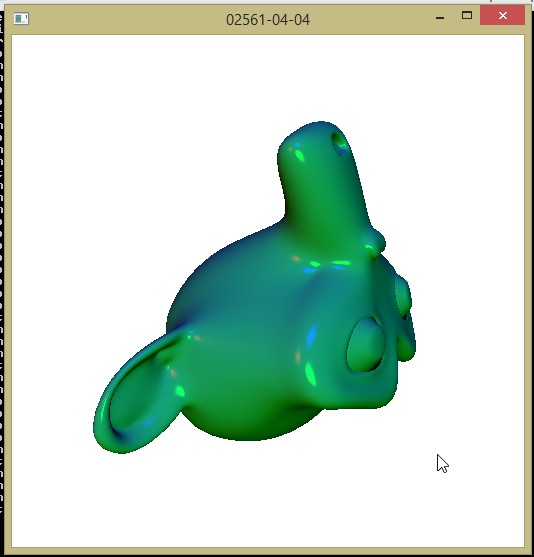
\includegraphics[width=0.75\textwidth]{figures/exercise_4_part_4}
	\end{center}
	\vspace{-4.5ex}\caption{Exercise 4 part 4 output}
	\label{fig:exercise_4_part_4} 
\end{figure}

\begin{lstlisting}[language=cpp, caption={Phong lightning}]
uniform mat4 ModelView;
uniform vec4 MaterialColor;
uniform vec4 MaterialSpecularColor;
uniform float Shininess;
#define MAX_LIGHTS 5
uniform int NumLights;
uniform struct Light {
	vec3 position;
	vec3 color;
	float lightType;
	float attenuation;
	float ambientCoefficient;
} Lights[MAX_LIGHTS];
in vec3 fragPosition;
in vec3 fragNormal;
out vec4 fragColor;

vec3 ApplyLight(Light light, vec3 normal, vec3 position)
{
	vec3 surfToLight = normalize(light.position);
	float attenuation = 1.0;
	if(light.lightType == 1.0)
	{
		surfToLight = normalize(light.position - position);
		float distance = length(light.position - position);
		attenuation = 1.0 / (1.0 + light.attenuation * pow(distance, 2));
	}
	vec3 surfToCamera = normalize(position);
	vec3 reflection = reflect(surfToLight, normal);
	vec3 ambient = light.ambientCoefficient * MaterialColor.xyz * light.color;
	float diffuseCoefficient = clamp(max(dot(normal, surfToLight), 0.0), 0.0, 1.0);
	vec3 diffuse = diffuseCoefficient * MaterialColor.xyz * light.color;
	float specularCoefficient = diffuseCoefficient > 0 ? clamp(pow(max(dot(reflection, surfToCamera), 0.0), Shininess), 0.0, 1.0) : 0.0;
	vec3 specular = specularCoefficient * MaterialSpecularColor.xyz * light.color;
	return ambient + attenuation*(diffuse + specular);
}

void main() 
{ 
	vec3 normal = normalize(transpose(inverse(mat3(ModelView))) * fragNormal);
	vec3 position = vec3(ModelView * vec4(fragPosition, 1.0));
	vec3 linearColor = vec3(0);
	for(int i = 0; i < NumLights; ++i)
		linearColor += ApplyLight(Lights[i], normal, position);
	fragColor = vec4(linearColor, 1.0);
} 
\end{lstlisting}


\chapter{Exercise 5}
The purpose of the exercise is to get acquainted with input and
window management in Glut and OpenGL. In particular we will
work with mouse input, keyboard input, menus, multiple windows,
logic operations, selection and picking.

\section{Part 1}
	Pick function is choosing which type of object will be drawn, basing on
	a position of a mouse.
\section{Part 2}
	Performing a selection required following steps:
	\begin{enumerate}
	\item Build a texture
	\item Bind a texture to a frame buffer object
	\item Render the scene to a FBO with ids encoded as colors
	\item When click event is called, decode a pixel color on mouse position using FBO
	\item Decoded value is an object id
	\end{enumerate}	 
\section{Part 3}
I made a program, which can draw and edit simple circuit diagrams. My sample
diagram can be seen in the figure \ref{fig:exercise_5_part_3}.
\begin{figure}[ht!]
	\begin{center}
		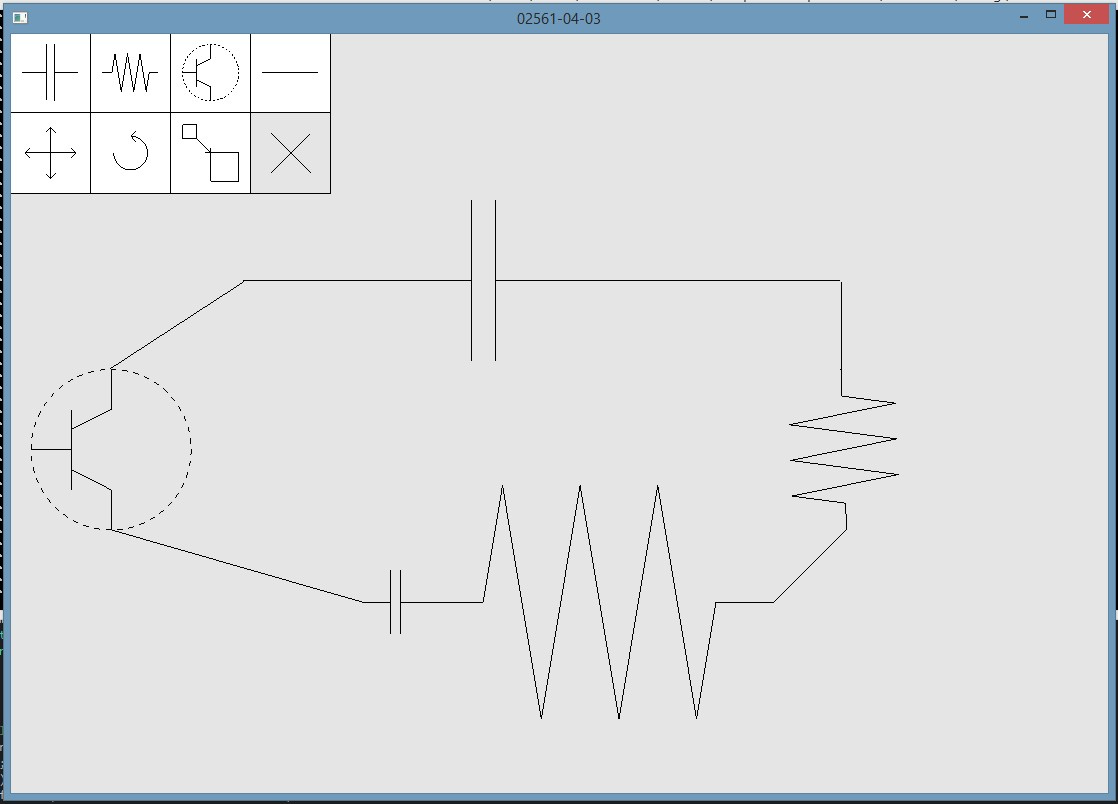
\includegraphics[width=1.0\textwidth]{figures/exercise_5_part_3}
	\end{center}
	\vspace{-4.5ex}\caption{Exercise 5 part 3 output}
	\label{fig:exercise_5_part_3} 
\end{figure}
\chapter{Exercise 5}
The purpose of the exercise is to understand the principles of 2D
texture mapping and how it can be used for polygon meshes.
Furthermore, the purpose of the exercise is to understand the
process of hidden surface removal and back-face culling.

\section{Part 1}
Hidden surface removal uses z-buffer to update the color of a pixel. Below
we can see two pictures of a scene rendered with and without depth test.

\begin{figure}[ht!]
	\begin{center}
		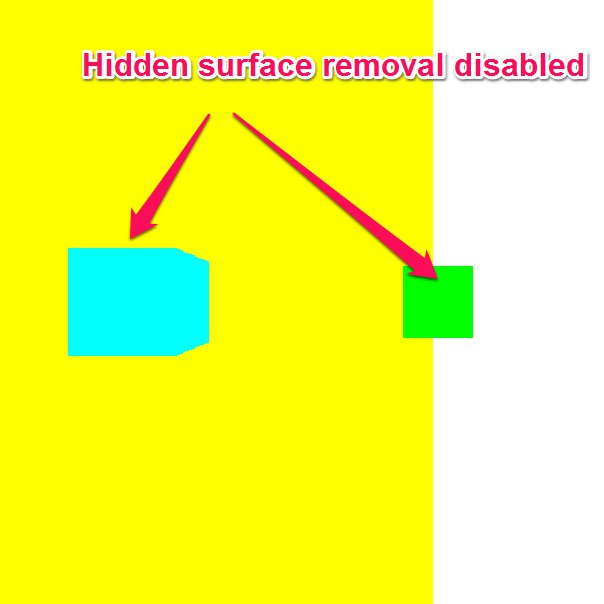
\includegraphics[width=0.28\textwidth]{figures/exercise_6_part_1_1}
	\end{center}
	\vspace{-4.5ex}\caption{Exercise 6 part 1-1 output}
	\label{fig:exercise_6_part_1_1} 
\end{figure}
\begin{figure}[ht!]
	\begin{center}
		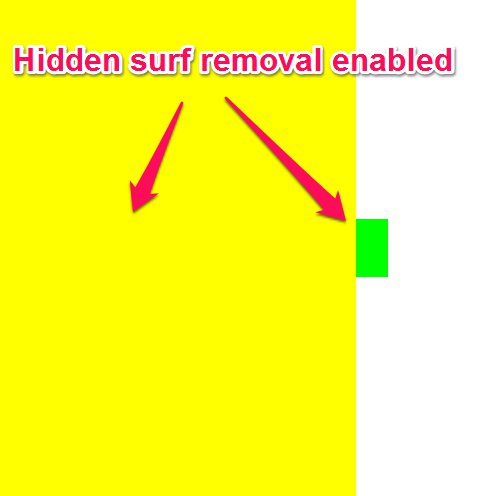
\includegraphics[width=0.28\textwidth]{figures/exercise_6_part_1_2}
	\end{center}
	\vspace{-4.5ex}\caption{Exercise 6 part 1-2 output}
	\label{fig:exercise_6_part_1_2} 
\end{figure}

OpenGL makes use of normal vector to the surface and its angle with camera view direction
to judge if the surface is front or back facing. Below we can see some screenshots
with various culling modes.

\begin{figure}[ht!]
	\begin{center}
		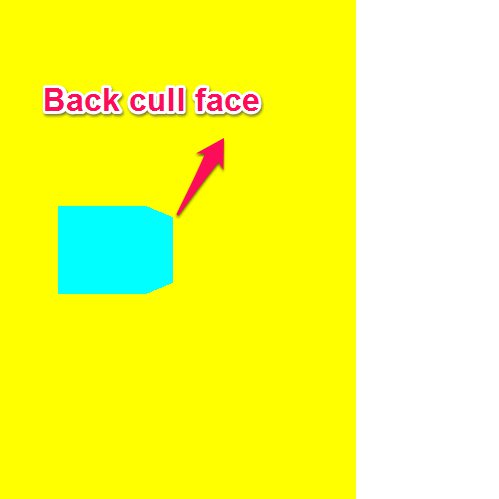
\includegraphics[width=0.3\textwidth]{figures/exercise_6_part_2_1}
	\end{center}
	\vspace{-4.5ex}\caption{Exercise 6 part 2-3 output}
	\label{fig:exercise_6_part_2_1} 
\end{figure}
\begin{figure}[ht!]
	\begin{center}
		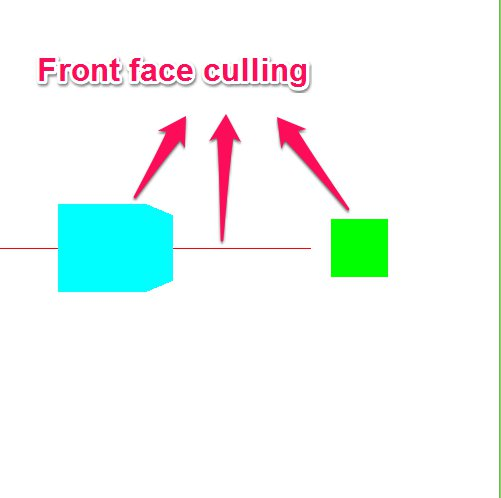
\includegraphics[width=0.3\textwidth]{figures/exercise_6_part_2_2}
	\end{center}
	\vspace{-4.5ex}\caption{Exercise 6 part 1-4 output}
	\label{fig:exercise_6_part_2_2} 
\end{figure}
\begin{figure}[ht!]
	\begin{center}
		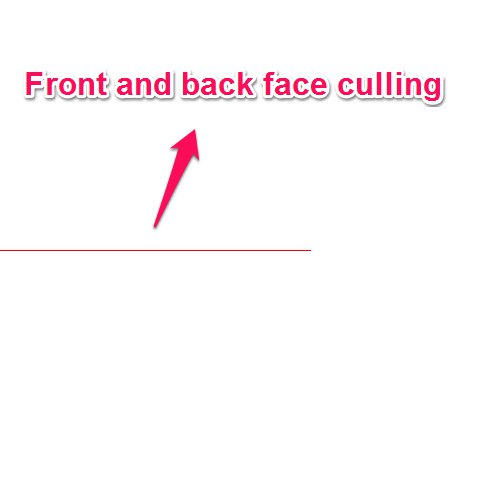
\includegraphics[width=0.3\textwidth]{figures/exercise_6_part_2_3}
	\end{center}
	\vspace{-4.5ex}\caption{Exercise 6 part 1-5 output}
	\label{fig:exercise_6_part_2_3} 
\end{figure}
\clearpage

\section{Part 2}
Using a near frustum value of $9.5$ and far value of $11.0$ with angle of 30 degrees 
I obtained parts of front and back of teapot clipped away. The results are in the figure
\ref{fig:exercise_6_part_3}

\begin{figure}[ht!]
	\begin{center}
		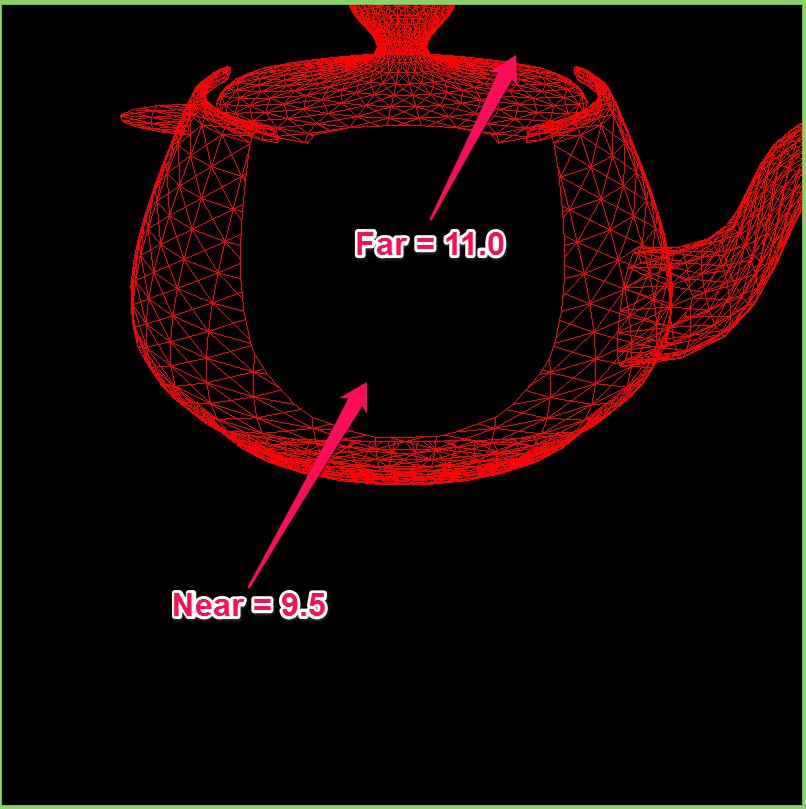
\includegraphics[width=1.0\textwidth]{figures/exercise_6_part_3}
	\end{center}
	\vspace{-4.5ex}\caption{Exercise 6 part 2 output}
	\label{fig:exercise_6_part_3} 
\end{figure}
\clearpage

\section{Part 3}
Using function glTexParameteri I obtained different texture filter techniques as it can
be seen in figures below.

\begin{figure}[ht!]
	\begin{center}
		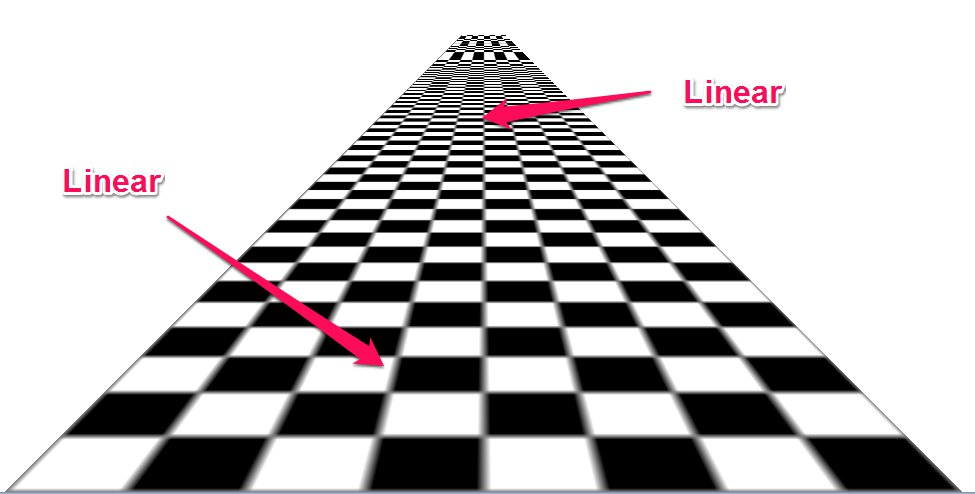
\includegraphics[width=0.45\textwidth]{figures/exercise_6_part_4_1}
	\end{center}
	\vspace{-4.5ex}\caption{Exercise 6 part 3-1 output}
	\label{fig:exercise_6_part_4_1} 
\end{figure}
\begin{figure}[ht!]
	\begin{center}
		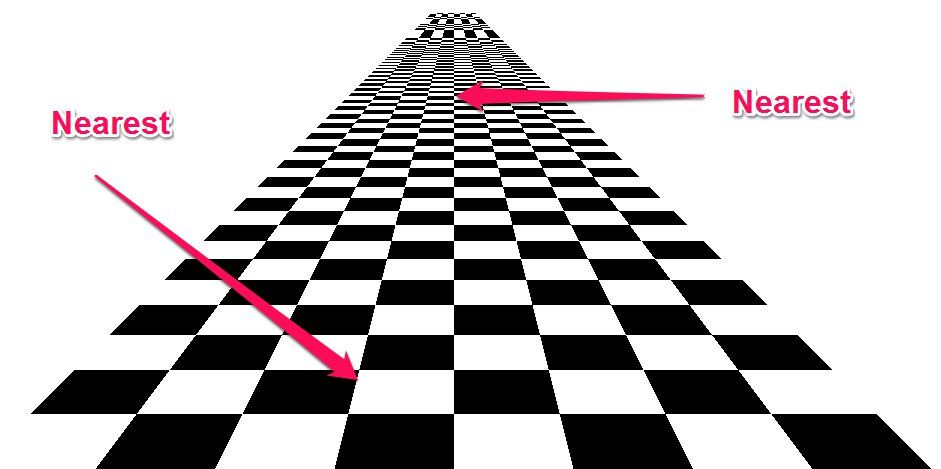
\includegraphics[width=0.45\textwidth]{figures/exercise_6_part_4_2}
	\end{center}
	\vspace{-4.5ex}\caption{Exercise 6 part 3-2 output}
	\label{fig:exercise_6_part_4_2} 
\end{figure}
\begin{figure}[ht!]
	\begin{center}
		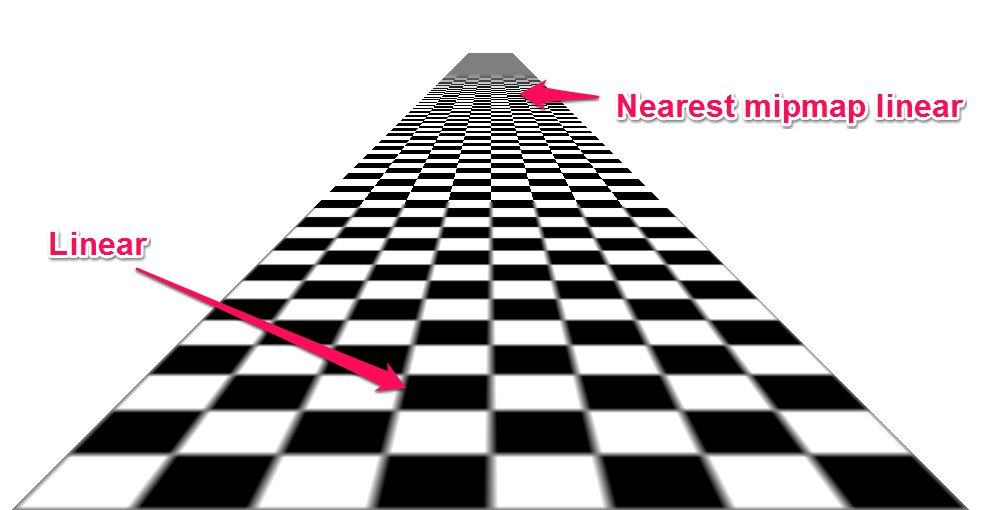
\includegraphics[width=0.45\textwidth]{figures/exercise_6_part_4_3}
	\end{center}
	\vspace{-4.5ex}\caption{Exercise 6 part 3-3 output}
	\label{fig:exercise_6_part_4_3} 
\end{figure}
\begin{figure}[ht!]
	\begin{center}
		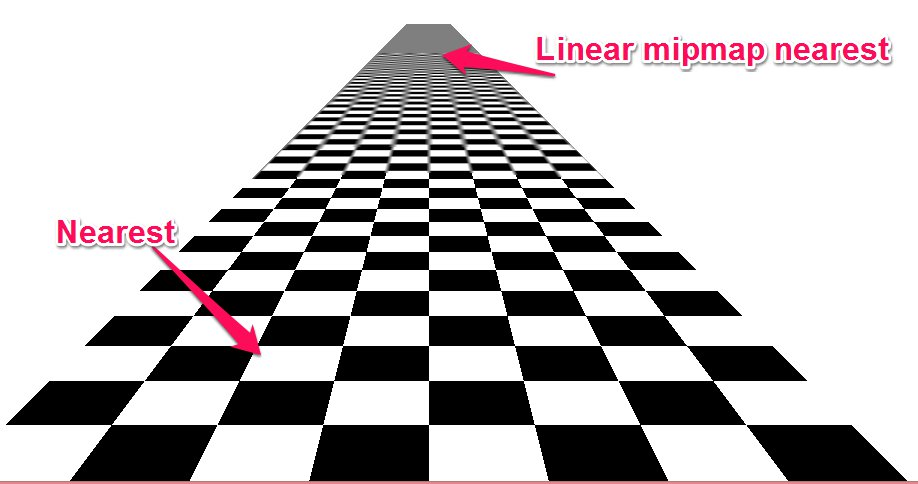
\includegraphics[width=0.45\textwidth]{figures/exercise_6_part_4_4}
	\end{center}
	\vspace{-4.5ex}\caption{Exercise 6 part 3-4 output}
	\label{fig:exercise_6_part_4_4} 
\end{figure}

\section{Part 4}
After modification of polygon and texture vertices I got results shown below for
several configurations of texture wrapping.

\begin{figure}[ht!]
	\begin{center}
		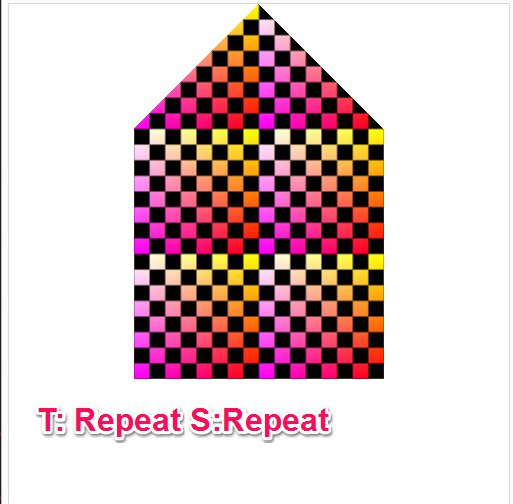
\includegraphics[width=0.35\textwidth]{figures/exercise_6_part_5_1}
	\end{center}
	\vspace{-4.5ex}\caption{Exercise 6 part 4-1 output}
	\label{fig:exercise_6_part_5_1} 
\end{figure}
\begin{figure}[ht!]
	\begin{center}
		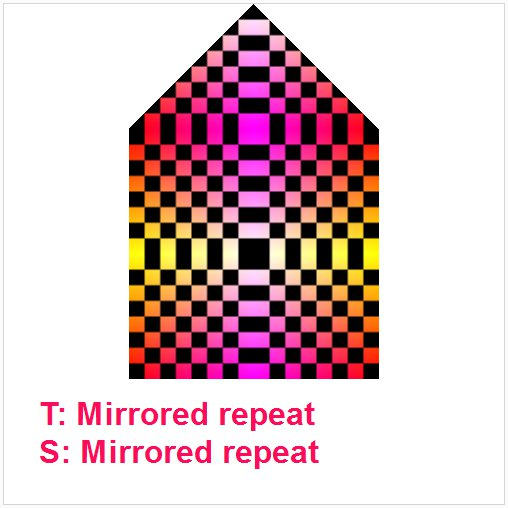
\includegraphics[width=0.35\textwidth]{figures/exercise_6_part_5_2}
	\end{center}
	\vspace{-4.5ex}\caption{Exercise 6 part 4-3 output}
	\label{fig:exercise_6_part_5_3} 
\end{figure}
\begin{figure}[ht!]
	\begin{center}
		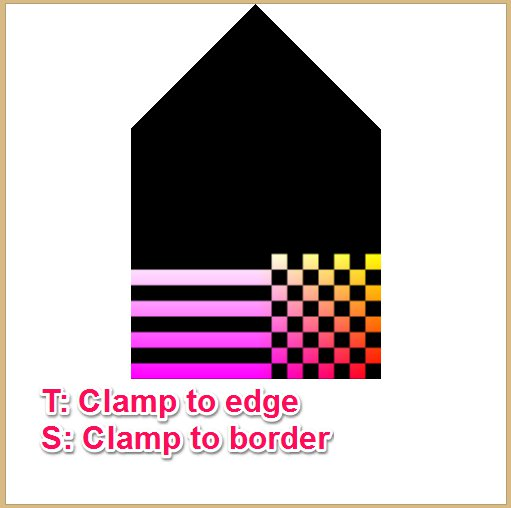
\includegraphics[width=0.35\textwidth]{figures/exercise_6_part_5_3}
	\end{center}
	\vspace{-4.5ex}\caption{Exercise 6 part 4-3 output}
	\label{fig:exercise_6_part_5_3} 
\end{figure}


\section{Part 5 and 6}
I succeded in making an animated texture assigning a transformation matrix of
rotation to a textureTrans uniform and multiplying texture coordinates with
that matrix. 
\begin{lstlisting}[language=cpp, caption={Texture animation - main.cpp}]
mat4 textureTrans = RotateZ(rotation);
glUniformMatrix4fv(textureTransUniform, 1, GL_TRUE, textureTrans);
\end{lstlisting}
\begin{lstlisting}[language=cpp, caption={Texture animation - tex-shader.vert}]
vTextureCoord = (textureTrans * vec4(textureCoord,0.0,1.0)).xy;
\end{lstlisting}
I obtained results which can be seen in the figure \ref{fig:exercise_6_part_6}
\begin{figure}[ht!]
	\begin{center}
		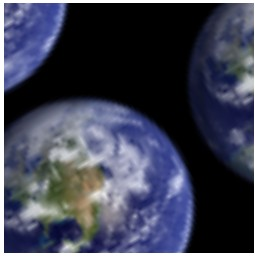
\includegraphics[width=.8\textwidth]{figures/exercise_6_part_6}
	\end{center}
	\vspace{-4.5ex}\caption{Exercise 6 part 5 and 6 output}
	\label{fig:exercise_6_part_6} 
\end{figure}

%----------------------------------------------------------------------------------------
%	BIBLIOGRAPHY
%----------------------------------------------------------------------------------------

\bibliographystyle{apalike}
\nocite{*}
\bibliography{references}

%----------------------------------------------------------------------------------------


\end{document}